% Options for packages loaded elsewhere
\PassOptionsToPackage{unicode}{hyperref}
\PassOptionsToPackage{hyphens}{url}
%
\documentclass[
]{article}
\usepackage{amsmath,amssymb}
\usepackage{iftex}
\ifPDFTeX
  \usepackage[T1]{fontenc}
  \usepackage[utf8]{inputenc}
  \usepackage{textcomp} % provide euro and other symbols
\else % if luatex or xetex
  \usepackage{unicode-math} % this also loads fontspec
  \defaultfontfeatures{Scale=MatchLowercase}
  \defaultfontfeatures[\rmfamily]{Ligatures=TeX,Scale=1}
\fi
\usepackage{lmodern}
\ifPDFTeX\else
  % xetex/luatex font selection
\fi
% Use upquote if available, for straight quotes in verbatim environments
\IfFileExists{upquote.sty}{\usepackage{upquote}}{}
\IfFileExists{microtype.sty}{% use microtype if available
  \usepackage[]{microtype}
  \UseMicrotypeSet[protrusion]{basicmath} % disable protrusion for tt fonts
}{}
\makeatletter
\@ifundefined{KOMAClassName}{% if non-KOMA class
  \IfFileExists{parskip.sty}{%
    \usepackage{parskip}
  }{% else
    \setlength{\parindent}{0pt}
    \setlength{\parskip}{6pt plus 2pt minus 1pt}}
}{% if KOMA class
  \KOMAoptions{parskip=half}}
\makeatother
\usepackage{xcolor}
\usepackage[margin=1in]{geometry}
\usepackage{color}
\usepackage{fancyvrb}
\newcommand{\VerbBar}{|}
\newcommand{\VERB}{\Verb[commandchars=\\\{\}]}
\DefineVerbatimEnvironment{Highlighting}{Verbatim}{commandchars=\\\{\}}
% Add ',fontsize=\small' for more characters per line
\usepackage{framed}
\definecolor{shadecolor}{RGB}{248,248,248}
\newenvironment{Shaded}{\begin{snugshade}}{\end{snugshade}}
\newcommand{\AlertTok}[1]{\textcolor[rgb]{0.94,0.16,0.16}{#1}}
\newcommand{\AnnotationTok}[1]{\textcolor[rgb]{0.56,0.35,0.01}{\textbf{\textit{#1}}}}
\newcommand{\AttributeTok}[1]{\textcolor[rgb]{0.13,0.29,0.53}{#1}}
\newcommand{\BaseNTok}[1]{\textcolor[rgb]{0.00,0.00,0.81}{#1}}
\newcommand{\BuiltInTok}[1]{#1}
\newcommand{\CharTok}[1]{\textcolor[rgb]{0.31,0.60,0.02}{#1}}
\newcommand{\CommentTok}[1]{\textcolor[rgb]{0.56,0.35,0.01}{\textit{#1}}}
\newcommand{\CommentVarTok}[1]{\textcolor[rgb]{0.56,0.35,0.01}{\textbf{\textit{#1}}}}
\newcommand{\ConstantTok}[1]{\textcolor[rgb]{0.56,0.35,0.01}{#1}}
\newcommand{\ControlFlowTok}[1]{\textcolor[rgb]{0.13,0.29,0.53}{\textbf{#1}}}
\newcommand{\DataTypeTok}[1]{\textcolor[rgb]{0.13,0.29,0.53}{#1}}
\newcommand{\DecValTok}[1]{\textcolor[rgb]{0.00,0.00,0.81}{#1}}
\newcommand{\DocumentationTok}[1]{\textcolor[rgb]{0.56,0.35,0.01}{\textbf{\textit{#1}}}}
\newcommand{\ErrorTok}[1]{\textcolor[rgb]{0.64,0.00,0.00}{\textbf{#1}}}
\newcommand{\ExtensionTok}[1]{#1}
\newcommand{\FloatTok}[1]{\textcolor[rgb]{0.00,0.00,0.81}{#1}}
\newcommand{\FunctionTok}[1]{\textcolor[rgb]{0.13,0.29,0.53}{\textbf{#1}}}
\newcommand{\ImportTok}[1]{#1}
\newcommand{\InformationTok}[1]{\textcolor[rgb]{0.56,0.35,0.01}{\textbf{\textit{#1}}}}
\newcommand{\KeywordTok}[1]{\textcolor[rgb]{0.13,0.29,0.53}{\textbf{#1}}}
\newcommand{\NormalTok}[1]{#1}
\newcommand{\OperatorTok}[1]{\textcolor[rgb]{0.81,0.36,0.00}{\textbf{#1}}}
\newcommand{\OtherTok}[1]{\textcolor[rgb]{0.56,0.35,0.01}{#1}}
\newcommand{\PreprocessorTok}[1]{\textcolor[rgb]{0.56,0.35,0.01}{\textit{#1}}}
\newcommand{\RegionMarkerTok}[1]{#1}
\newcommand{\SpecialCharTok}[1]{\textcolor[rgb]{0.81,0.36,0.00}{\textbf{#1}}}
\newcommand{\SpecialStringTok}[1]{\textcolor[rgb]{0.31,0.60,0.02}{#1}}
\newcommand{\StringTok}[1]{\textcolor[rgb]{0.31,0.60,0.02}{#1}}
\newcommand{\VariableTok}[1]{\textcolor[rgb]{0.00,0.00,0.00}{#1}}
\newcommand{\VerbatimStringTok}[1]{\textcolor[rgb]{0.31,0.60,0.02}{#1}}
\newcommand{\WarningTok}[1]{\textcolor[rgb]{0.56,0.35,0.01}{\textbf{\textit{#1}}}}
\usepackage{graphicx}
\makeatletter
\def\maxwidth{\ifdim\Gin@nat@width>\linewidth\linewidth\else\Gin@nat@width\fi}
\def\maxheight{\ifdim\Gin@nat@height>\textheight\textheight\else\Gin@nat@height\fi}
\makeatother
% Scale images if necessary, so that they will not overflow the page
% margins by default, and it is still possible to overwrite the defaults
% using explicit options in \includegraphics[width, height, ...]{}
\setkeys{Gin}{width=\maxwidth,height=\maxheight,keepaspectratio}
% Set default figure placement to htbp
\makeatletter
\def\fps@figure{htbp}
\makeatother
\setlength{\emergencystretch}{3em} % prevent overfull lines
\providecommand{\tightlist}{%
  \setlength{\itemsep}{0pt}\setlength{\parskip}{0pt}}
\setcounter{secnumdepth}{-\maxdimen} % remove section numbering
\ifLuaTeX
  \usepackage{selnolig}  % disable illegal ligatures
\fi
\usepackage{bookmark}
\IfFileExists{xurl.sty}{\usepackage{xurl}}{} % add URL line breaks if available
\urlstyle{same}
\hypersetup{
  hidelinks,
  pdfcreator={LaTeX via pandoc}}

\author{}
\date{\vspace{-2.5em}}

\begin{document}

\newcommand\textpkg[1]{\textbf{\texttt{#1}}}

This chapter demonstrates the use of \textbf{\texttt{QTLExperiment}} and
\textbf{\texttt{multistateQTL}} with data from the GTEx Consortium,
version 8 \autocite{GTEx_2020}. The GTEx consortium includes
\emph{cis}-eQTL data from 38 tissue types. This chapter interweaves text
and R code and output to provide as comprehensive a demonstration as
possible of the use of the packages for the analysis of multi-state eQTL
data.

\section{Installing packages}\label{installing-packages}

The \textbf{\texttt{QTLExperiment}} and \textbf{\texttt{multistateQTL}}
packages are available on Bioconductor. To install
\textbf{\texttt{QTLExperiment}}, Bioconductor version 3.18 or later is
required, and for \textbf{\texttt{multistateQTL}} version 3.19 or later
is required. The code to install these packages from within R is shown
below.

\footnotesize

\begin{Shaded}
\begin{Highlighting}[]
\ControlFlowTok{if}\NormalTok{ (}\SpecialCharTok{!}\FunctionTok{require}\NormalTok{(}\StringTok{"BiocManager"}\NormalTok{, }\AttributeTok{quietly=}\ConstantTok{TRUE}\NormalTok{))}
    \FunctionTok{install.packages}\NormalTok{(}\StringTok{"BiocManager"}\NormalTok{)}

\NormalTok{BiocManager}\SpecialCharTok{::}\FunctionTok{install}\NormalTok{(}\StringTok{"QTLExperiment"}\NormalTok{)}
\NormalTok{BiocManager}\SpecialCharTok{::}\FunctionTok{install}\NormalTok{(}\StringTok{"multistateQTL"}\NormalTok{)}
\end{Highlighting}
\end{Shaded}

\normalsize

Once the packages are installed, it is simple to load the packages into
R. \footnotesize

\begin{Shaded}
\begin{Highlighting}[]
\FunctionTok{library}\NormalTok{(QTLExperiment)}
\FunctionTok{library}\NormalTok{(multistateQTL)}
\end{Highlighting}
\end{Shaded}

\normalsize

\section{Loading data}\label{loading-data}

The data for this section can be downloaded from the
\href{https://www.gtexportal.org/home/downloads/adult-gtex/qtl}{GTEx Portal}.
The download link has file name \emph{``GTEx\_Analysis\_v8\_eQTL.tar''}.
For each state, the file was extracted. I selected 14 tissue types that
have at least 200 samples to be used for this demonstration.

The \texttt{sumstats2qtle()} function is used to load the data by
providing a data frame with the state names and file paths, and
information about the relevant columns in the summary statistic files.
For the first argument, we provide a data frame with two columns,
\texttt{state} and \texttt{path}. This data frame lists the name of each
state in the analysis and the file path to summary statistics for that
state. We also supply the the names of the columns to use for the
feature IDs, variant IDs, effect sizes, standard errors, and p-values.

\footnotesize

\begin{Shaded}
\begin{Highlighting}[]
\NormalTok{input\_path }\OtherTok{\textless{}{-}} \StringTok{"GTEx/data/"}

\NormalTok{state }\OtherTok{\textless{}{-}} \FunctionTok{c}\NormalTok{(}\StringTok{"Muscle\_Skeletal"}\NormalTok{, }\StringTok{"Whole\_Blood"}\NormalTok{, }\StringTok{"Skin\_Sun\_Exposed\_Lower\_leg"}\NormalTok{, }
    \StringTok{"Adipose\_Subcutaneous"}\NormalTok{, }\StringTok{"Thyroid"}\NormalTok{, }\StringTok{"Lung"}\NormalTok{, }\StringTok{"Cells\_Cultured\_fibroblasts"}\NormalTok{, }
    \StringTok{"Stomach"}\NormalTok{, }\StringTok{"Pancreas"}\NormalTok{, }\StringTok{"Pituitary"}\NormalTok{, }\StringTok{"Spleen"}\NormalTok{, }\StringTok{"Liver"}\NormalTok{, }\StringTok{"Brain\_Cerebellum"}\NormalTok{,}
    \StringTok{"Brain\_Cortex"}\NormalTok{)}

\NormalTok{input }\OtherTok{\textless{}{-}} \FunctionTok{data.frame}\NormalTok{(}
    \AttributeTok{state=}\NormalTok{state,}
    \AttributeTok{path=}\FunctionTok{paste0}\NormalTok{(input\_path, state, }\StringTok{".v8.egenes.txt"}\NormalTok{))}

\NormalTok{qtle }\OtherTok{\textless{}{-}} \FunctionTok{sumstats2qtle}\NormalTok{(}
\NormalTok{    input,}
    \AttributeTok{feature\_id=}\StringTok{"gene\_id"}\NormalTok{,}
    \AttributeTok{variant\_id=}\StringTok{"variant\_id"}\NormalTok{,}
    \AttributeTok{betas=}\StringTok{"slope"}\NormalTok{,}
    \AttributeTok{errors=}\StringTok{"slope\_se"}\NormalTok{,}
    \AttributeTok{pvalues=}\StringTok{"pval\_nominal"}\NormalTok{)}
\end{Highlighting}
\end{Shaded}

\begin{Shaded}
\begin{Highlighting}[]
\NormalTok{qtle}
\end{Highlighting}
\end{Shaded}

\begin{verbatim}
## class: QTLExperiment 
## dim: 298068 14 
## metadata(0):
## assays(3): betas errors pvalues
## rownames(298068): ENSG00000227232.5|chr1_666028_G_A_b38
##   ENSG00000268903.1|chr1_933869_T_C_b38 ...
##   ENSG00000124333.15|chrX_155744353_G_T_b38
##   ENSG00000185203.12|chrX_156003173_A_C_b38
## rowData names(2): variant_id feature_id
## colnames(14): Muscle_Skeletal Whole_Blood ... Brain_Cerebellum
##   Brain_Cortex
## colData names(1): state_id
\end{verbatim}

\normalsize

\section{Basic operations}\label{basic-operations}

We can view basic properties of the \texttt{QTLExperiment} object such
as the number of rows (\texttt{nrows}), number of columns
(\texttt{ncols}), and the dimensions (\texttt{dim}). This shows that the
object contains 298068 association tests, across 14 states.

\footnotesize

\begin{Shaded}
\begin{Highlighting}[]
\FunctionTok{dim}\NormalTok{(qtle)}
\end{Highlighting}
\end{Shaded}

\begin{verbatim}
## [1] 298068     14
\end{verbatim}

\normalsize

We can use the \texttt{state\_id()} setter to change the state IDs, for
example to make them shorter. Feature IDs or variant IDs can also be
updated if needed using the \texttt{feature\_id()} or
\texttt{variant\_id()} functions. This process will also update the
information in all other aspects of the \texttt{QTLExperiment} object,
such as in the assays, rowData and colData.

\footnotesize

\begin{Shaded}
\begin{Highlighting}[]
\FunctionTok{state\_id}\NormalTok{(qtle)}
\end{Highlighting}
\end{Shaded}

\begin{verbatim}
##  [1] "Muscle_Skeletal"            "Whole_Blood"               
##  [3] "Skin_Sun_Exposed_Lower_leg" "Adipose_Subcutaneous"      
##  [5] "Thyroid"                    "Lung"                      
##  [7] "Cells_Cultured_fibroblasts" "Stomach"                   
##  [9] "Pancreas"                   "Pituitary"                 
## [11] "Spleen"                     "Liver"                     
## [13] "Brain_Cerebellum"           "Brain_Cortex"
\end{verbatim}

\begin{Shaded}
\begin{Highlighting}[]
\FunctionTok{state\_id}\NormalTok{(qtle) }\OtherTok{\textless{}{-}}  \FunctionTok{c}\NormalTok{(}\StringTok{"Muscle"}\NormalTok{, }\StringTok{"Blood"}\NormalTok{, }\StringTok{"Skin"}\NormalTok{, }\StringTok{"Adipose"}\NormalTok{, }\StringTok{"Thyroid"}\NormalTok{, }\StringTok{"Lung"}\NormalTok{,}
    \StringTok{"Fibroblast"}\NormalTok{, }\StringTok{"Stomach"}\NormalTok{, }\StringTok{"Pancreas"}\NormalTok{, }\StringTok{"Pituitary"}\NormalTok{, }\StringTok{"Spleen"}\NormalTok{, }\StringTok{"Liver"}\NormalTok{, }
    \StringTok{"Brain\_Cerebellum"}\NormalTok{, }\StringTok{"Brain\_Cortex"}\NormalTok{)}
\FunctionTok{state\_id}\NormalTok{(qtle)}
\end{Highlighting}
\end{Shaded}

\begin{verbatim}
##  [1] "Muscle"           "Blood"            "Skin"             "Adipose"         
##  [5] "Thyroid"          "Lung"             "Fibroblast"       "Stomach"         
##  [9] "Pancreas"         "Pituitary"        "Spleen"           "Liver"           
## [13] "Brain_Cerebellum" "Brain_Cortex"
\end{verbatim}

\normalsize

The \texttt{betas()}, \texttt{errors()} and \texttt{pvalues()} functions
can be used to view the numeric matrices stored in these assays. In the
code below I have subset to show a small portion of the effect sizes
from the summary statistics data.

\footnotesize

\begin{Shaded}
\begin{Highlighting}[]
\FunctionTok{betas}\NormalTok{(qtle)[}\DecValTok{1}\SpecialCharTok{:}\DecValTok{5}\NormalTok{, }\DecValTok{1}\SpecialCharTok{:}\DecValTok{4}\NormalTok{]}
\end{Highlighting}
\end{Shaded}

\begin{verbatim}
##                                          Muscle     Blood      Skin   Adipose
## ENSG00000227232.5|chr1_666028_G_A_b38  0.439049  0.489662        NA        NA
## ENSG00000268903.1|chr1_933869_T_C_b38  0.783867        NA        NA        NA
## ENSG00000269981.1|chr1_933869_T_C_b38  0.773216        NA        NA        NA
## ENSG00000279457.4|chr1_599167_G_A_b38 -0.534898 -0.544131 -0.527948 -0.687794
## ENSG00000228463.9|chr1_281912_C_G_b38  0.439693        NA        NA        NA
\end{verbatim}

\normalsize

We can add additional columns to the colData of the \texttt{qtle} object
using the ``\$'' accessor. This can be any type of vector (logical,
numeric, character) provided the length of the vector is equal to the
number of states in the \texttt{qtle} object. I have added a grouping of
the tissues which does not distinguish between the two types of brain
tissues, for use in later visualisations. The colData will automatically
update to reflect the additional column.

\footnotesize

\begin{Shaded}
\begin{Highlighting}[]
\NormalTok{qtle}\SpecialCharTok{$}\NormalTok{broad\_type }\OtherTok{\textless{}{-}} \FunctionTok{c}\NormalTok{(}\StringTok{"Muscle"}\NormalTok{, }\StringTok{"Blood"}\NormalTok{, }\StringTok{"Skin"}\NormalTok{, }\StringTok{"Adipose"}\NormalTok{, }\StringTok{"Thyroid"}\NormalTok{, }\StringTok{"Lung"}\NormalTok{,}
    \StringTok{"Fibroblast"}\NormalTok{, }\StringTok{"Stomach"}\NormalTok{, }\StringTok{"Pancreas"}\NormalTok{, }\StringTok{"Pituitary"}\NormalTok{, }\StringTok{"Spleen"}\NormalTok{, }\StringTok{"Liver"}\NormalTok{, }
    \StringTok{"Brain"}\NormalTok{, }\StringTok{"Brain"}\NormalTok{)}
\FunctionTok{colData}\NormalTok{(qtle)}
\end{Highlighting}
\end{Shaded}

\begin{verbatim}
## DataFrame with 14 rows and 2 columns
##                          state_id  broad_type
##                       <character> <character>
## Muscle                     Muscle      Muscle
## Blood                       Blood       Blood
## Skin                         Skin        Skin
## Adipose                   Adipose     Adipose
## Thyroid                   Thyroid     Thyroid
## ...                           ...         ...
## Pituitary               Pituitary   Pituitary
## Spleen                     Spleen      Spleen
## Liver                       Liver       Liver
## Brain_Cerebellum Brain_Cerebellum       Brain
## Brain_Cortex         Brain_Cortex       Brain
\end{verbatim}

\normalsize

It may be of interest to look at the number of genes that are included
in the analysis. While the number of rows corresponds to Gene:SNP pairs,
we can obtain this quantity using the \texttt{feature\_id()} accessor.

\footnotesize

\begin{Shaded}
\begin{Highlighting}[]
\FunctionTok{head}\NormalTok{(}\FunctionTok{rowData}\NormalTok{(qtle))}
\end{Highlighting}
\end{Shaded}

\begin{verbatim}
## DataFrame with 6 rows and 2 columns
##                                                 variant_id         feature_id
##                                                <character>        <character>
## ENSG00000227232.5|chr1_666028_G_A_b38  chr1_666028_G_A_b38  ENSG00000227232.5
## ENSG00000268903.1|chr1_933869_T_C_b38  chr1_933869_T_C_b38  ENSG00000268903.1
## ENSG00000269981.1|chr1_933869_T_C_b38  chr1_933869_T_C_b38  ENSG00000269981.1
## ENSG00000279457.4|chr1_599167_G_A_b38  chr1_599167_G_A_b38  ENSG00000279457.4
## ENSG00000228463.9|chr1_281912_C_G_b38  chr1_281912_C_G_b38  ENSG00000228463.9
## ENSG00000237094.11|chr1_887001_C_T_b38 chr1_887001_C_T_b38 ENSG00000237094.11
\end{verbatim}

\begin{Shaded}
\begin{Highlighting}[]
\FunctionTok{length}\NormalTok{(}\FunctionTok{unique}\NormalTok{(}\FunctionTok{feature\_id}\NormalTok{(qtle)))}
\end{Highlighting}
\end{Shaded}

\begin{verbatim}
## [1] 33579
\end{verbatim}

\normalsize

This data set has 298068 rows of associations across 33579 genes.
\footnotesize

\normalsize

\section{Manipulate and Filter}\label{manipulate-and-filter}

\subsection{Dealing with missing data}\label{dealing-with-missing-data}

It is common for there to be NA values in multi-state QTL data, as we
are looking for associations between SNPs and gene expression across
many states. The \texttt{getComplete()} function retains only the rows
with values in at least 90\% of the states (since we have specified
\texttt{n=0.9}) .

\footnotesize

\normalsize

\footnotesize

\begin{Shaded}
\begin{Highlighting}[]
\NormalTok{qtle\_na }\OtherTok{\textless{}{-}} \FunctionTok{getComplete}\NormalTok{(qtle, }\AttributeTok{n=}\FloatTok{0.9}\NormalTok{, }\AttributeTok{verbose=}\ConstantTok{TRUE}\NormalTok{)}
\end{Highlighting}
\end{Shaded}

\begin{verbatim}
## Removing 278841 tests with NAs in >= 13 states...
\end{verbatim}

\begin{Shaded}
\begin{Highlighting}[]
\FunctionTok{dim}\NormalTok{(qtle\_na)}
\end{Highlighting}
\end{Shaded}

\begin{verbatim}
## [1] 19227    14
\end{verbatim}

\normalsize

We have removed tests which have NA values in 1 or more of the 14 states
(\(\lceil0.9\times 14\rceil = 13\) complete values needed). This results
in 19227 rows of association tests.

The \texttt{replaceNAs()} function is used to replace NA values in the
data using the default method for imputing values. The benefit of
imputing data instead of retaining only complete rows is that we can
keep more rows of association tests. \footnotesize

\begin{Shaded}
\begin{Highlighting}[]
\NormalTok{qtle\_na }\OtherTok{\textless{}{-}} \FunctionTok{replaceNAs}\NormalTok{(qtle\_na)}
\end{Highlighting}
\end{Shaded}

\normalsize

Following NA removal and replacement we can see that there are no NA
effect sizes, and the effect sizes that were previously NA are now 0.
\footnotesize

\begin{Shaded}
\begin{Highlighting}[]
\FunctionTok{head}\NormalTok{(}\FunctionTok{betas}\NormalTok{(qtle\_na))[}\DecValTok{1}\SpecialCharTok{:}\DecValTok{5}\NormalTok{, }\DecValTok{1}\SpecialCharTok{:}\DecValTok{4}\NormalTok{]}
\end{Highlighting}
\end{Shaded}

\begin{verbatim}
##                                           Muscle     Blood      Skin   Adipose
## ENSG00000227232.5|chr1_666028_G_A_b38   0.439049  0.489662  0.000000  0.000000
## ENSG00000279457.4|chr1_599167_G_A_b38  -0.534898 -0.544131 -0.527948 -0.687794
## ENSG00000225972.1|chr1_1543591_G_T_b38 -0.799339  0.000000  0.000000 -0.700075
## ENSG00000228327.3|chr1_806017_A_G_b38  -0.746695  0.000000  0.000000  0.000000
## ENSG00000237491.8|chr1_818228_T_A_b38   1.134340  0.000000  0.000000  0.000000
\end{verbatim}

\normalsize

\section{Calculations}\label{calculations}

\subsection{Calling significance}\label{calling-significance}

The \texttt{callSignificance()} function can be used to determine which
tests are significant for each state. This function creates a new assay
called \texttt{significant} which has the same dimensions as the
\emph{betas}, \emph{errors}, and p-values assays. There are options in
this function to perform feature-wise and global multiple-testing
correction, but since the p-values provided by the GTEx Consortium have
already been adjusted, we will use the \texttt{simple} mode.
\footnotesize

\begin{Shaded}
\begin{Highlighting}[]
\NormalTok{qtle\_na }\OtherTok{\textless{}{-}} \FunctionTok{callSignificance}\NormalTok{(qtle\_na, }\AttributeTok{assay=}\StringTok{"pvalues"}\NormalTok{, }\AttributeTok{thresh=}\FloatTok{0.05}\NormalTok{)}
\end{Highlighting}
\end{Shaded}

\normalsize

We use the \texttt{getSignificant()} function to subset the
\textbf{\texttt{QTLExperiment}} object to only rows with at least one
significant test.

\footnotesize

\begin{Shaded}
\begin{Highlighting}[]
\NormalTok{qtle\_sig }\OtherTok{\textless{}{-}} \FunctionTok{getSignificant}\NormalTok{(qtle\_na)}
\end{Highlighting}
\end{Shaded}

\normalsize

\section{Visualisations}\label{visualisations}

\subsection{Plotting global sharing}\label{plotting-global-sharing}

The function \texttt{runPairwiseSharing()} is used to calculate the
amount of sharing of QTLs between each pair of states. This information
is added to the metadata of the \textbf{\texttt{QTLExperiment}} object,
where it can be viewed directly or visualised using
\texttt{plotPairwiseSharing()}. The plot shows that there are some
states with a higher level of sharing than others, for example states
`Brain\_Cortex' and `Brain\_Cerebellum' have over 20\% of eQTLs in
common, as do states `Skin' and `Adipose'.

\footnotesize

\begin{Shaded}
\begin{Highlighting}[]
\NormalTok{qtle\_top }\OtherTok{\textless{}{-}} \FunctionTok{runPairwiseSharing}\NormalTok{(qtle\_sig)}

\CommentTok{\# Preview of pairwise sharing matrix}
\FunctionTok{metadata}\NormalTok{(qtle\_top)}\SpecialCharTok{$}\NormalTok{pairwiseSharing[}\DecValTok{1}\SpecialCharTok{:}\DecValTok{3}\NormalTok{, }\DecValTok{1}\SpecialCharTok{:}\DecValTok{6}\NormalTok{]}
\end{Highlighting}
\end{Shaded}

\begin{verbatim}
##            Muscle      Blood      Skin   Adipose    Thyroid      Lung
## Muscle 1.00000000 0.09711752 0.1583623 0.1776650 0.14985110 0.1402541
## Blood  0.09711752 1.00000000 0.1126816 0.1128954 0.09849952 0.1505861
## Skin   0.15836230 0.11268164 1.0000000 0.2357102 0.18777728 0.1770624
\end{verbatim}

\begin{Shaded}
\begin{Highlighting}[]
\CommentTok{\# Plot pairwise sharing}
\FunctionTok{plotPairwiseSharing}\NormalTok{(qtle\_top, }\AttributeTok{annotateColsBy=}\FunctionTok{c}\NormalTok{(}\StringTok{"nSignificant"}\NormalTok{, }\StringTok{"broad\_type"}\NormalTok{))}
\end{Highlighting}
\end{Shaded}

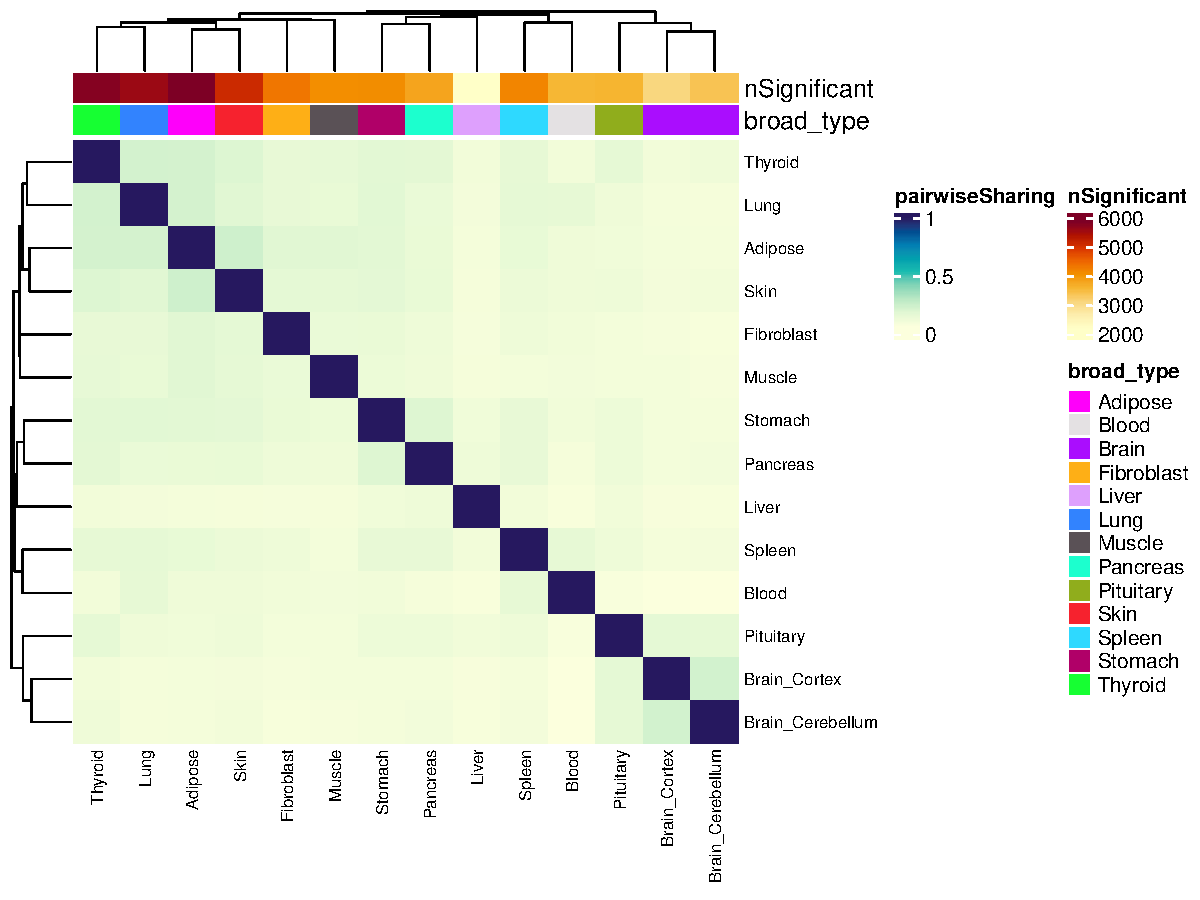
\includegraphics{GTEx_files/figure-latex/plot-pairwise-sharing-gtex-1.pdf}
\normalsize

\textbf{\texttt{QTLExperiment}} also contains a function to create an
UpSet plot. This function is based on the function
\texttt{ComplexHeatmap::UpSet()} but has been modified to support
\textbf{\texttt{QTLExperiment}} objects. An UpSet plot has a similar
function to a Venn Diagram, in that the goal is to visualise the number
of values in each combination of sets. The rows represent sets while the
columns list the possible combinations of these sets. Above the columns
there is a bar plot which shows the size of that combination of sets.
The columns are ordered in order of the most populated combination
through to the least, and combinations with 0 are not shown.

While a Venn Diagram is restricted to between 2 and 4 interacting sets,
an UpSet plot can depict many more sets. However, it can become
difficult to interpret these plots when there are more sets as there
will be many more columns. With \(n\) states, up to
\(\sum_{1}^n {n \choose i} = 2^n - 1\) columns may need to be plotted.
For example, with 5 states, up to 31 columns may be needed, depending on
the data set.

In \textbf{\texttt{QTLExperiment}}, UpSet plots are used as a way to
show the number of QTLs which are significant in multiple states. The
solid black circles and lines are used to indicate which combination of
tissue types is being measured, and the barplot above shows the number
of eQTLs in those states.

\footnotesize

\begin{Shaded}
\begin{Highlighting}[]
\NormalTok{qtle\_subset }\OtherTok{\textless{}{-}}\NormalTok{ qtle\_top[, }\FunctionTok{c}\NormalTok{(}\StringTok{"Muscle"}\NormalTok{, }\StringTok{"Lung"}\NormalTok{, }\StringTok{"Thyroid"}\NormalTok{, }\StringTok{"Spleen"}\NormalTok{, }\StringTok{"Blood"}\NormalTok{)]}

\FunctionTok{plotUpSet}\NormalTok{(qtle\_subset, }\AttributeTok{annotateColsBy=}\FunctionTok{c}\NormalTok{(}\StringTok{"nSignificant"}\NormalTok{, }\StringTok{"state\_id"}\NormalTok{))}
\end{Highlighting}
\end{Shaded}

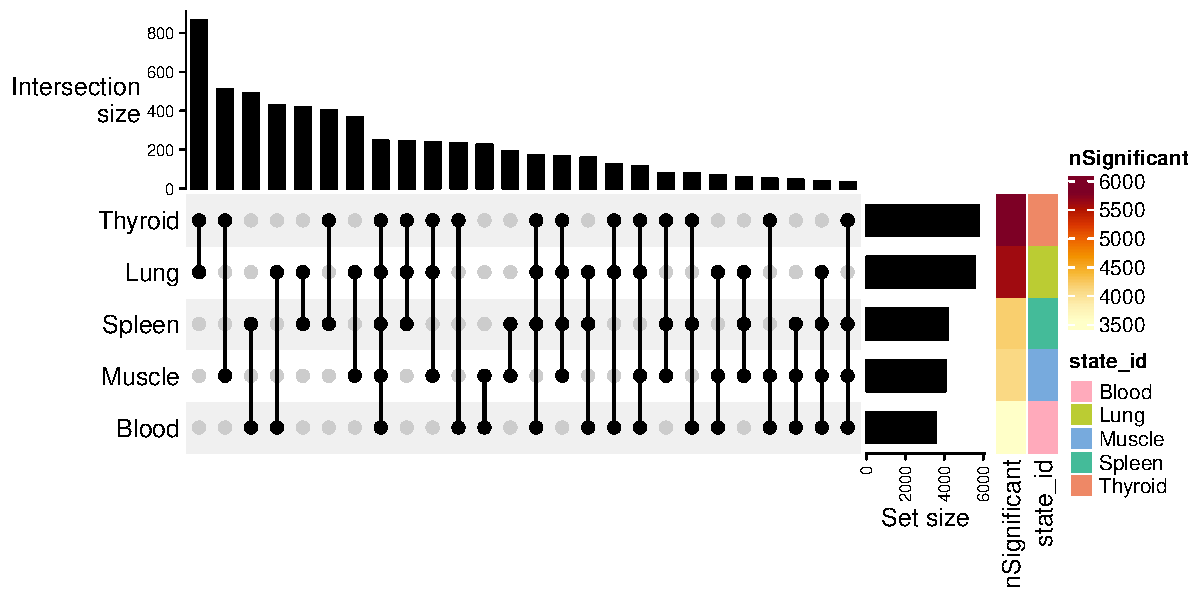
\includegraphics{GTEx_files/figure-latex/plot-upset-gtex-1.pdf}
\normalsize

\subsection{Characterizing multi-state QTL
patterns}\label{characterizing-multi-state-qtl-patterns}

The function \texttt{runTestMetrics()} characterises each test (row)
into categories including `global', `multistate' and `unique'. For more
detail, see section \ref{run_test_metrics}. This information is added
into the rowData of the QTLExperiment. \footnotesize

\begin{Shaded}
\begin{Highlighting}[]
\NormalTok{qtle\_top }\OtherTok{\textless{}{-}} \FunctionTok{runTestMetrics}\NormalTok{(qtle\_top)}

\FunctionTok{table}\NormalTok{(}\FunctionTok{rowData}\NormalTok{(qtle\_top)}\SpecialCharTok{$}\NormalTok{qtl\_type)}
\end{Highlighting}
\end{Shaded}

\begin{verbatim}
## 
##        global_shared multistate_diverging    multistate_shared 
##                   50                  507                18670
\end{verbatim}

\normalsize

The function \texttt{plotCompareStates()} visualises the multi-state
categories for two specified states, given as character vectors in
arguments \texttt{x} and \texttt{y}. The plot below shows that for the
states `Muscle' and `Blood', some tests are only significant in one
state, and a large number are shared, but there are very few diverging
eQTLs. A diverging eQTL has a different direction of effect on gene
expression in one state compared with another state. The output is shown
in figure \ref{plotCompareStates}. \footnotesize

\begin{Shaded}
\begin{Highlighting}[]
\FunctionTok{plotCompareStates}\NormalTok{(qtle\_top, }\AttributeTok{x=}\StringTok{"Muscle"}\NormalTok{, }\AttributeTok{y=}\StringTok{"Blood"}\NormalTok{)}\SpecialCharTok{$}\NormalTok{plot}
\end{Highlighting}
\end{Shaded}

\normalsize

\begin{figure}[h] 
\centering
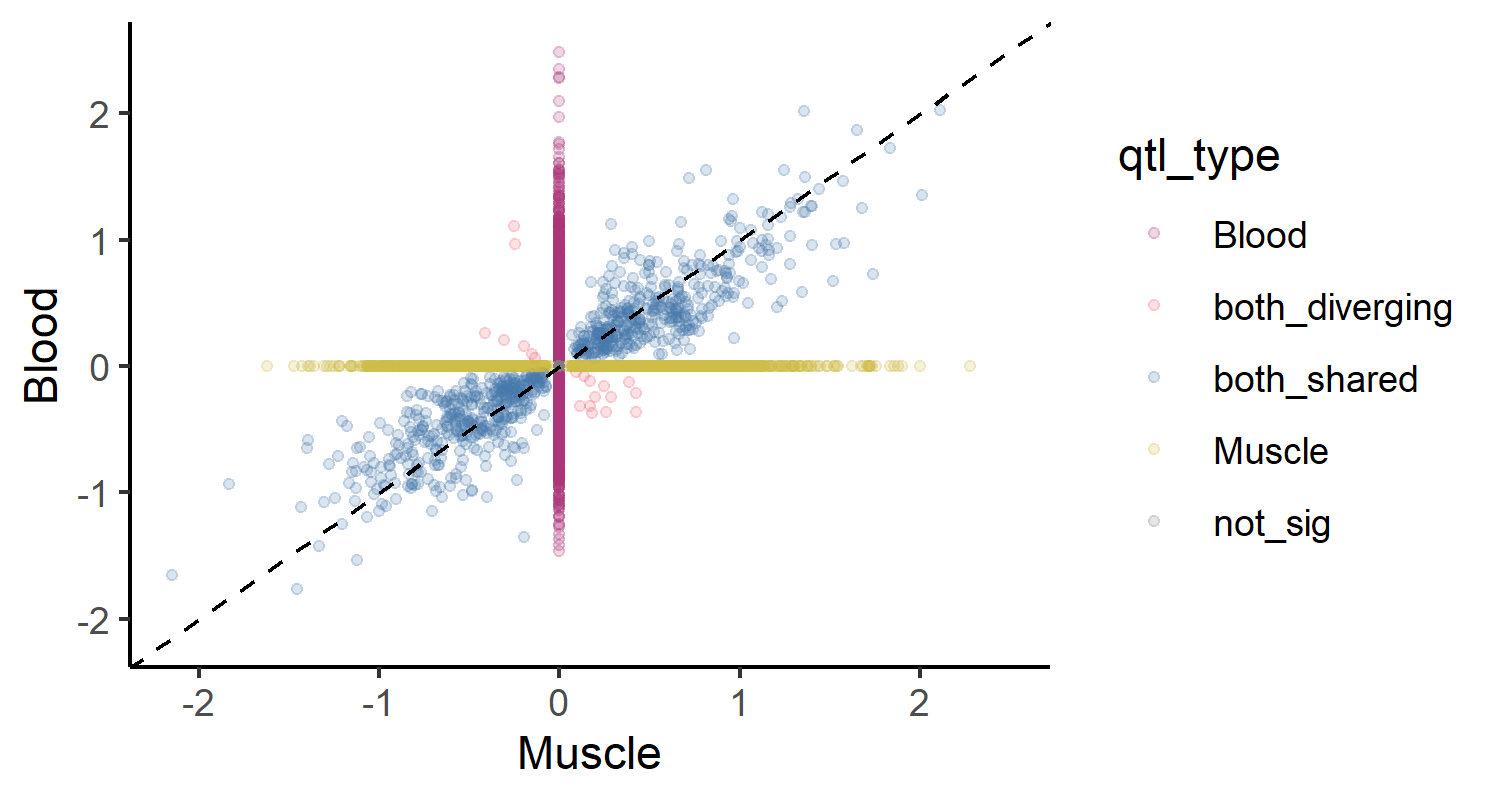
\includegraphics{Figures/plotCompareStates_gtex.png}
\caption{Output of the \texttt{plotCompareStates()} function.}
\label{plotCompareStates}
\end{figure}

The function \texttt{plotQTLClusters()} produces a heatmap of the data,
based on the \texttt{ComplexHeatmap::Heatmap()} function. Each row of
the heatmap corresponds to an association test (feature ID and variant
ID), and each column is a state. The colour value is determined by the
gene expression effect size for that state: colours close to white
indicate no change in gene expression for that state; red indicate that
the eQTL has a positive effect on gene expression in that state, and
blue values indicate the eQTL reduces the amount of gene expression.

The data has been filtered to select only rows which have an effect in
multiple states. I have also downsampled the data to 2000 rows to aid
visibility of the graph.

\footnotesize

\begin{Shaded}
\begin{Highlighting}[]
\NormalTok{qtle\_top\_ms }\OtherTok{\textless{}{-}} \FunctionTok{subset}\NormalTok{(qtle\_top, qtl\_type\_simple }\SpecialCharTok{==} \StringTok{"multistate"}\NormalTok{)}

\CommentTok{\# Downsample as there are 20,000 rows. }
\NormalTok{qtle\_ds }\OtherTok{\textless{}{-}}\NormalTok{ qtle\_top\_ms[}\FunctionTok{sample}\NormalTok{(}\FunctionTok{nrow}\NormalTok{(qtle\_top\_ms), }\DecValTok{2000}\NormalTok{), ]}

\FunctionTok{plotQTLClusters}\NormalTok{(}
\NormalTok{  qtle\_ds, }
  \AttributeTok{annotateColsBy=}\StringTok{"broad\_type"}\NormalTok{,}
  \AttributeTok{annotateRowsBy=}\FunctionTok{c}\NormalTok{(}\StringTok{"qtl\_type"}\NormalTok{))}
\end{Highlighting}
\end{Shaded}

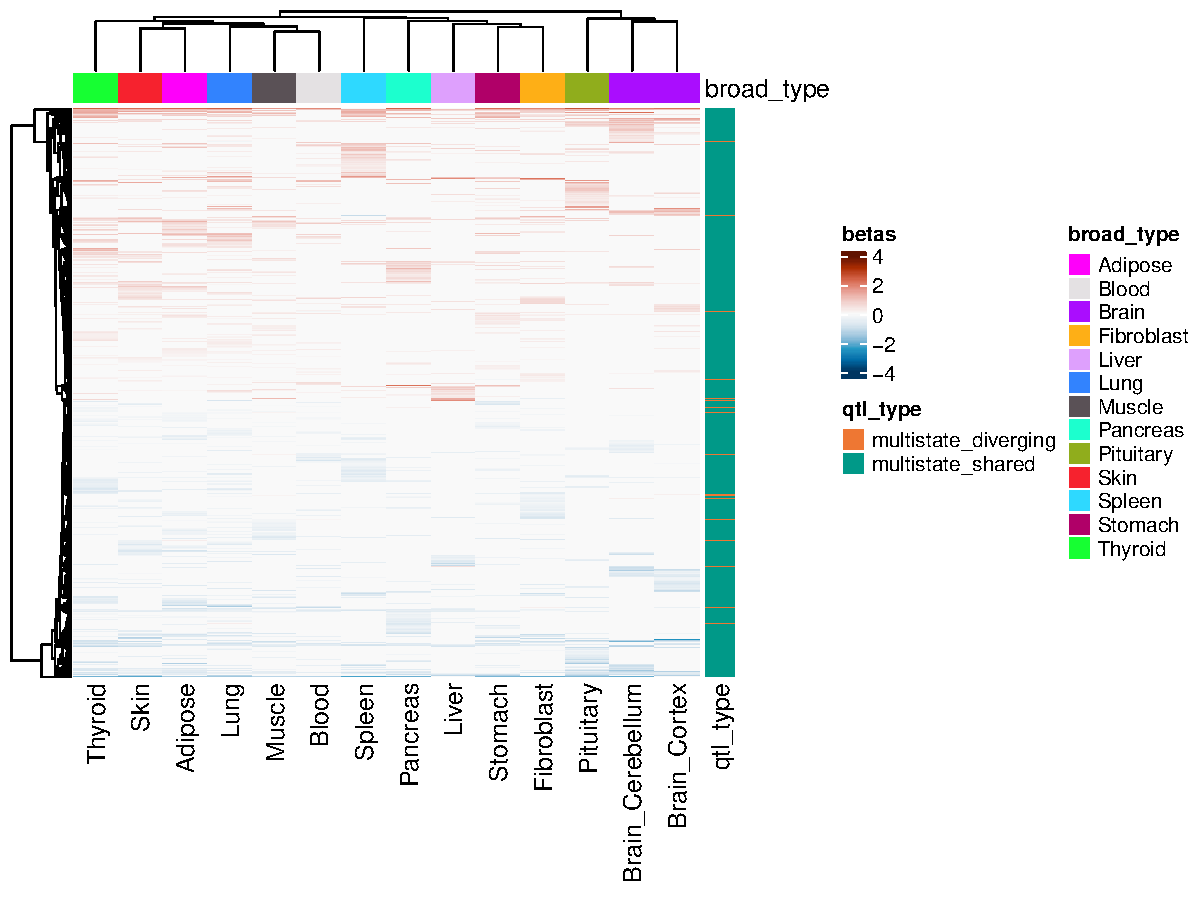
\includegraphics{GTEx_files/figure-latex/plot-qtl-clusters-gtex-1.pdf}
\normalsize

\section{Conclusion}\label{conclusion}

This chapter demonstrated the core functionality of the
\textbf{\texttt{QTLExperiment}} and \textbf{\texttt{multistateQTL}}
packages using a data set containing a number of different tissue types.
We covered functions which can be used to subset and manipulate the
data, perform calculations, identify significant tests, and visualise
various aspects of the data. In this chapter, the states we investigated
were tissues, which is clinical information that is known about the
samples from the beginning of the analysis. In the next chapter, we will
discuss a more detailed analysis involving single-cell data, where state
is `cell-type'.

\end{document}
